%!TEX program = xelatex

\documentclass[UTF8]{ctexart}
\usepackage{ctex}

\CTEXsetup[format={\Large\bfseries}]{section}

\usepackage[version=3]{mhchem} % Package for chemical equation typesetting
\usepackage{siunitx} % Provides the \SI{}{} and \si{} command for typesetting SI units
\usepackage{graphicx} % Required for the inclusion of images
% \graphicspath{{assets/}}
\usepackage{natbib} % Required to change bibliography style to APA
\usepackage{amsmath} % Required for some math elements 
\usepackage{amssymb}
\usepackage[hidelinks]{hyperref}
\usepackage{makecell} % 3 Packages for flexible tabular
\usepackage{multirow}
\usepackage{multicol}

\usepackage{pdfpages}  % include pdf pages for original data etc.

\usepackage{geometry}% 版面大小
\geometry{a4paper,scale=0.7}

\usepackage{fontspec}

\setCJKfamilyfont{hwxk}{STXingkai}% 字体
\newcommand{\hwxk}{\CJKfamily{hwxk}}

\usepackage{fancyhdr}% 页眉页脚
\fancypagestyle{EE_Digital1Exp_template}{
    \fancyhead[L]{\Large {\hwxk 南京大学电子科学与工程学院}}
    \fancyhead[R]{数字系统1实验报告}
    \fancyfoot[c]{- \thepage \ -}
    \renewcommand\footrulewidth{0pt}
}

% 4级目录
\setcounter{secnumdepth}{4}
\setcounter{tocdepth}{4}

\usepackage{graphicx} % Packages for figures
\usepackage{caption2}
\usepackage{subfigure}
\usepackage{float}


%设置图片、表格编号
\renewcommand{\thetable}{\thesubsection{}-\arabic{table}}
\renewcommand{\thefigure}{\thesubsection{}-\arabic{figure}}
\renewcommand{\thefigure}{\thesubsection{}-\arabic{equation}}
\usepackage{amsmath}
\numberwithin{figure}{subsection}
\numberwithin{table}{subsection}
\numberwithin{equation}{subsection}

\setlength\parindent{6pt} % Removes all indentation from paragraphs

\renewcommand{\labelenumi}{\alph{enumi}.} % Make numbering in the enumerate environment by letter rather than number (e.g. section 6)

%\usepackage{times} % Uncomment to use the Times New Roman font

%----------------------------------------------------------------------------------------
%	DOCUMENT INFORMATION
%----------------------------------------------------------------------------------------

\title{\textbf{实验三\ 移位寄存器}} % Title

\author{电子科学与工程学院\ 刘时宜\ 201180078} % Author name

\date{} % Date for the report

\begin{document}

\pagestyle{EE_Digital1Exp_template}

\maketitle % Insert the title, author and date

\begin{center}
    \begin{tabular}{l r}
    实验日期: & 2021年11月17日 \\ % Date the experiment was performed
     & 2021年11月24日 \\ % Date the experiment was performed
    指导老师: & 高健 % Instructor/supervisor
    \end{tabular}
    \par 点击目录、书签栏、以及行文中的图表标号的均可跳转至相应页面
    \end{center}
    
% If you wish to include an abstract, uncomment the lines below
% \begin{abstract}
% Abstract text
% \end{abstract}

\tableofcontents

\section{实验目的}
\begin{enumerate}
    \item 验证移位寄存器的功能
    \item 利用移位寄存器搭建数据收发器
\end{enumerate}

\section{实验仪器与主要器材}
\begin{center}
    \begin{tabular}{ll}
        \textbf{仪器:} & \\
        Basys3 FPGA 开发板 & 1台\\
        KEYSIGHT DSOX1102AG 示波器 & 1台\\
        示波器高频探头 & 1套\\
        ROGOL DM3068 万用表 & 1台\\
        \textbf{软件:} & \\
        Multisim & 14.1 \\
        Digilent Adept & 2.19.2 \\
        Vivado & 2015.4 \\
        \textbf{耗材:} & \\
        导线 & 若干 \\
    \end{tabular}
\end{center}

\section{实验原理}
\par 在各种复杂的数字电路中,不但需要对二值信号进行算术运算和逻辑运算,还经常需要将这些信号和运算结果保存下来。因此,需要使用具有记忆功能的基本逻辑单元。能够储存1位二值信号的基本单元电路统称触发器。
\par 寄存器用于储存一组二值代码,它被广泛运用于各类数字系统和数字计算机当中。因为一个触发器能够储存1位二值数据,所以用N个触发器组成的寄存器可以储存N位二进制代码。
\par 移位寄存器除了具有储存代码的功能以外,还具有移位功能。所谓移位功能,是指寄存器里储存的代码能够在移位脉冲的作用下依次左移或者右移。因此,移位寄存器不但可以用来寄存代码,还可以用来实现数据的串行-并行转换、数值的运算以及数据处理等。

\section{实验过程}
\subsection{移位寄存器单源周期触发测试}
\par 实验电路如图\ref{single source citcuit}所示。将已经编译好的bit文件下载到开发板上,观察实验现象。

\begin{figure}[H]
    \begin{center}
        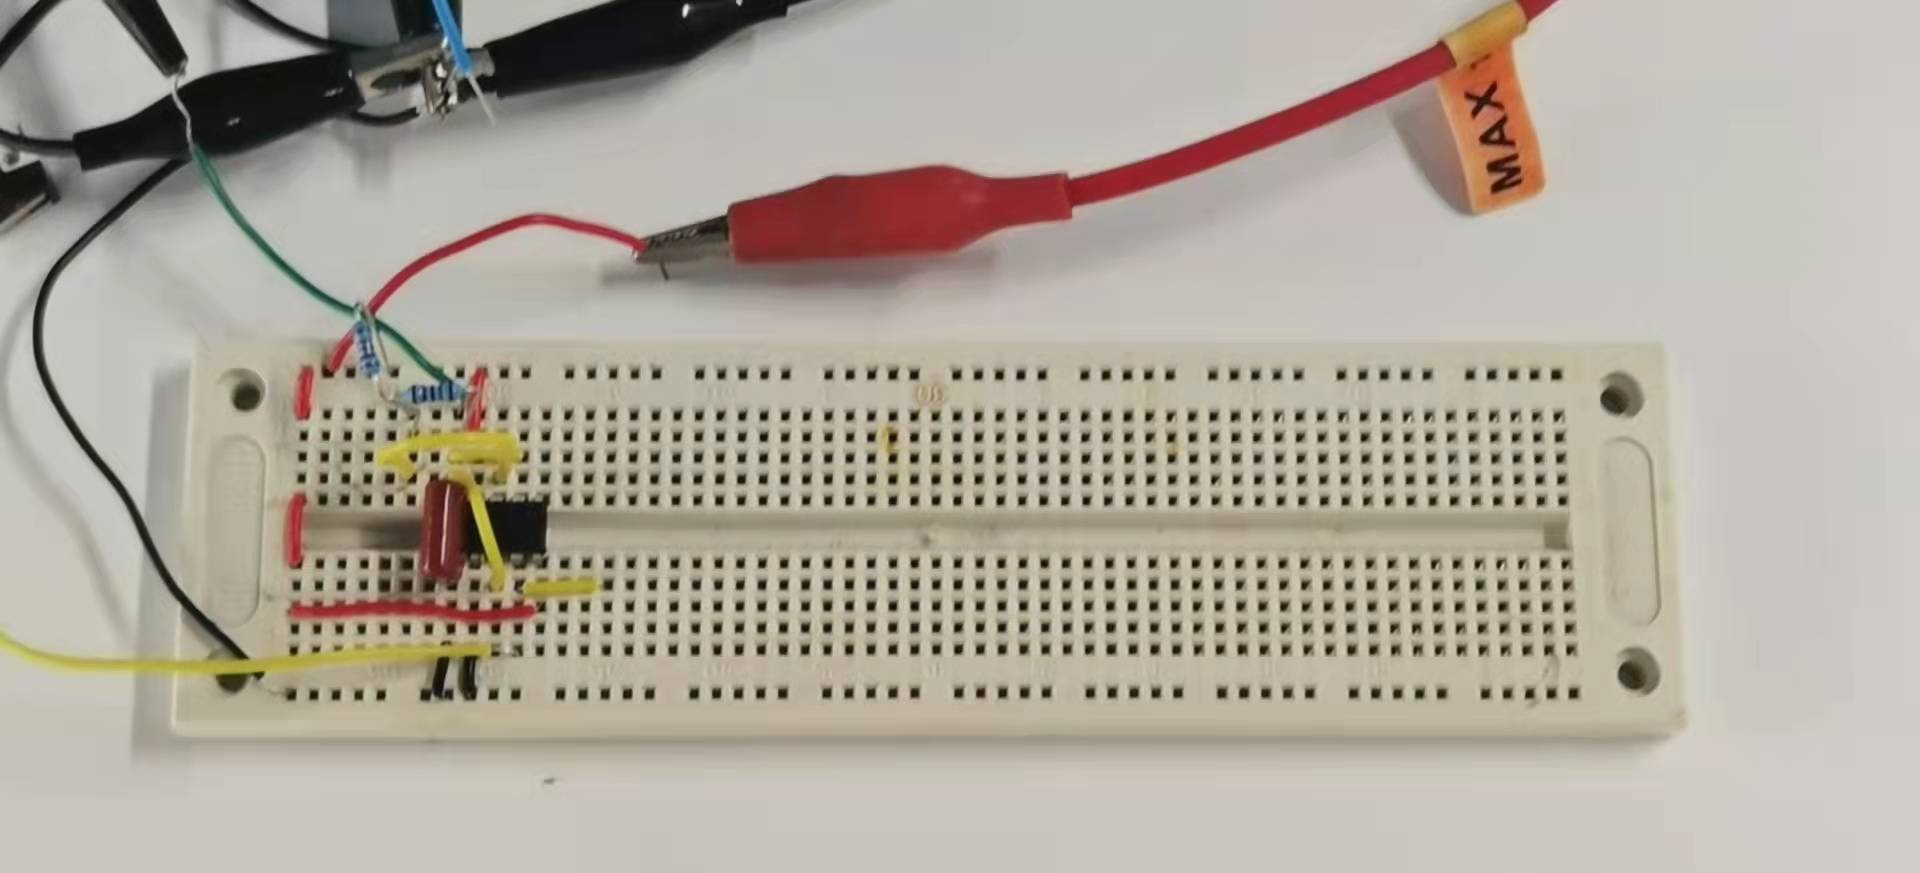
\includegraphics[width=0.8\textwidth]{pics/1S-V2/circuit.jpg}
    \end{center}
    \caption{移位寄存器单源周期触发测试电路}
    \label{single source citcuit}
\end{figure}

\subsubsection{实验结果}
使用示波器测量引脚JB0与JB2的波形图\ref{1S-V2 osci}所示:
\begin{figure}[H]
    \centering
    \subfigure[SW1]{
    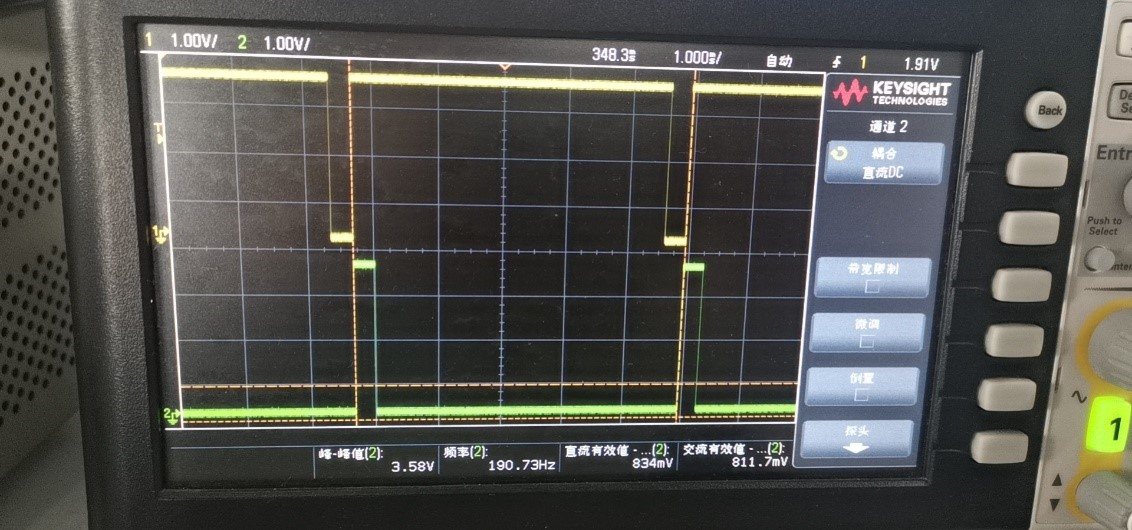
\includegraphics[width=0.45\textwidth]{pics/1S-V2/1.jpg}}
    \subfigure[SW2]{
    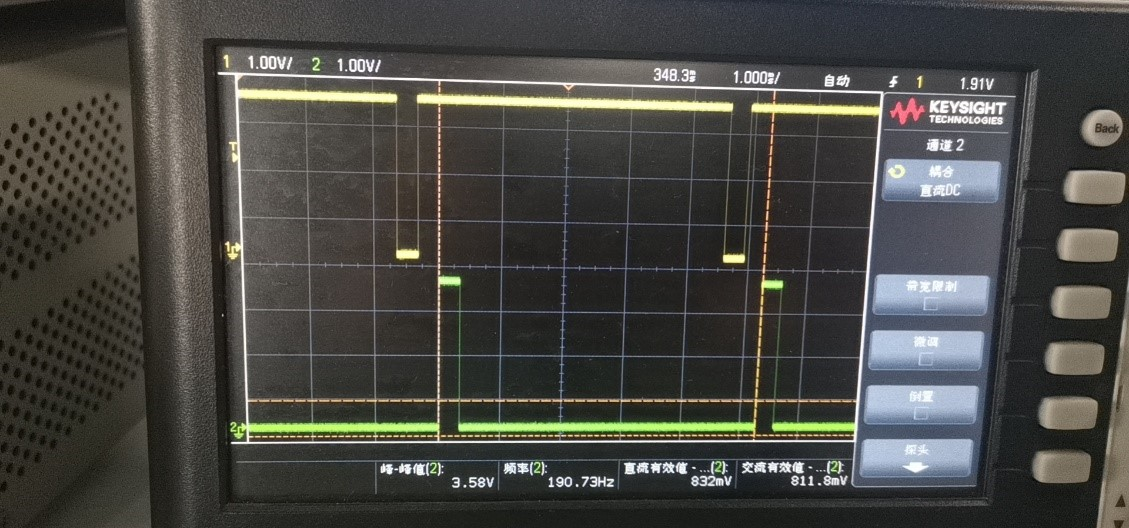
\includegraphics[width=0.45\textwidth]{pics/1S-V2/2.jpg}}
    \subfigure[SW3]{
    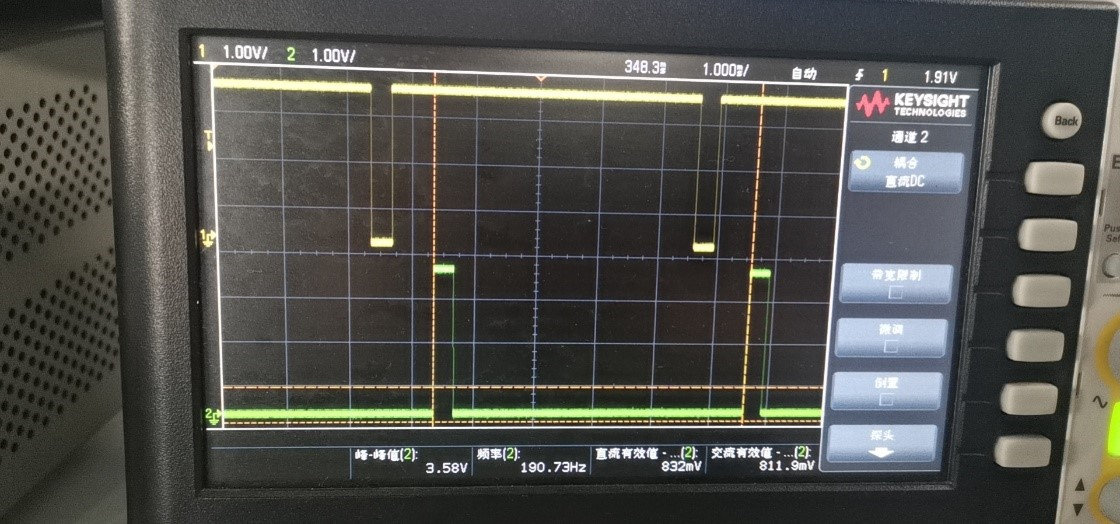
\includegraphics[width=0.45\textwidth]{pics/1S-V2/3.jpg}}
    \subfigure[SW4]{
    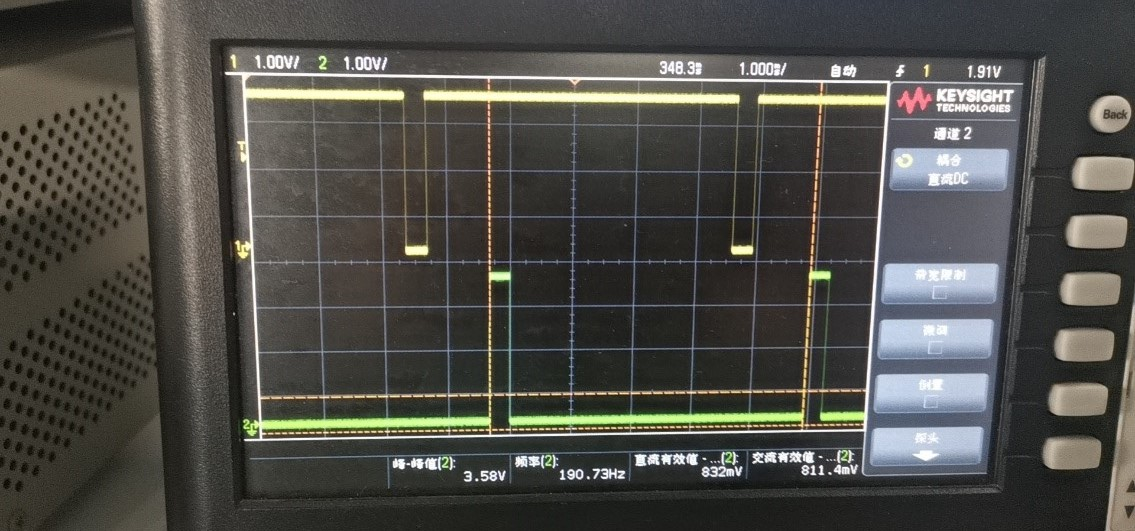
\includegraphics[width=0.45\textwidth]{pics/1S-V2/4.jpg}}
    \subfigure[SW2、SW6]{
    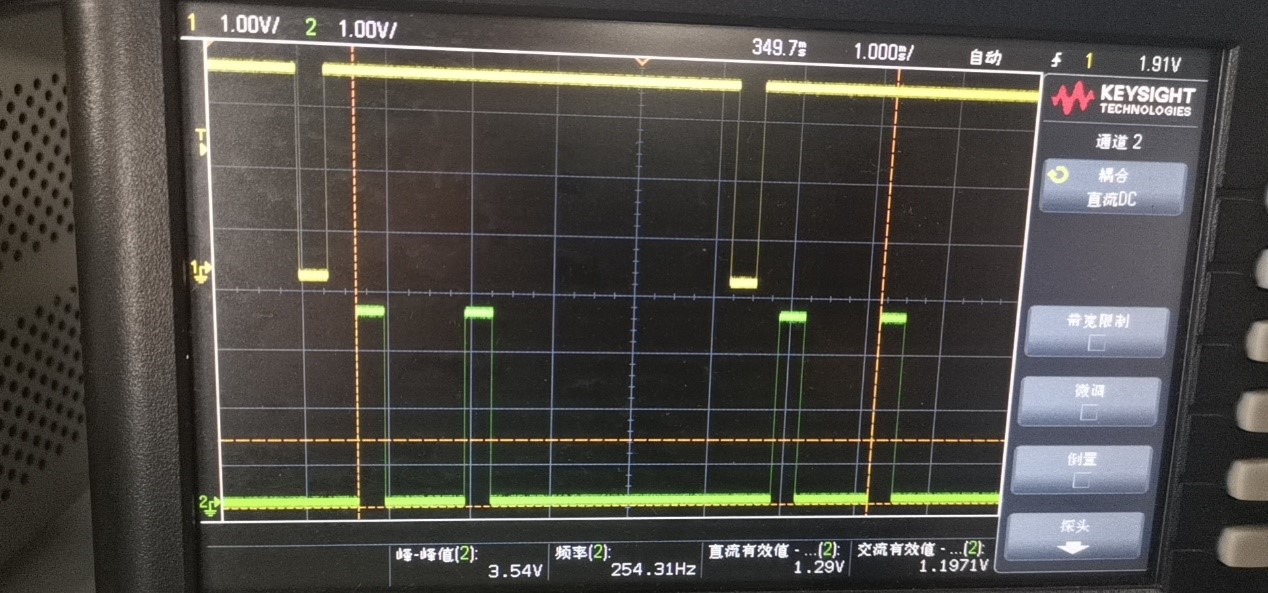
\includegraphics[width=0.45\textwidth]{pics/1S-V2/26.jpg}}
    \subfigure[SW0、SW2、SW6]{
    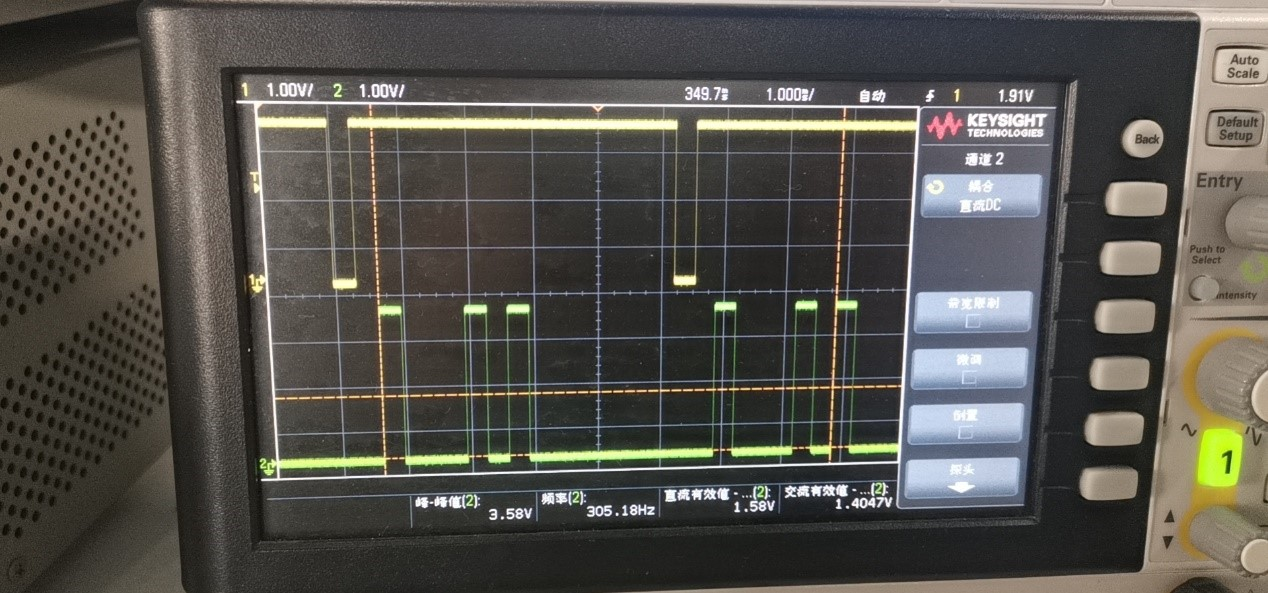
\includegraphics[width=0.45\textwidth]{pics/1S-V2/026.jpg}}
    \subfigure[SW7、SW8]{
    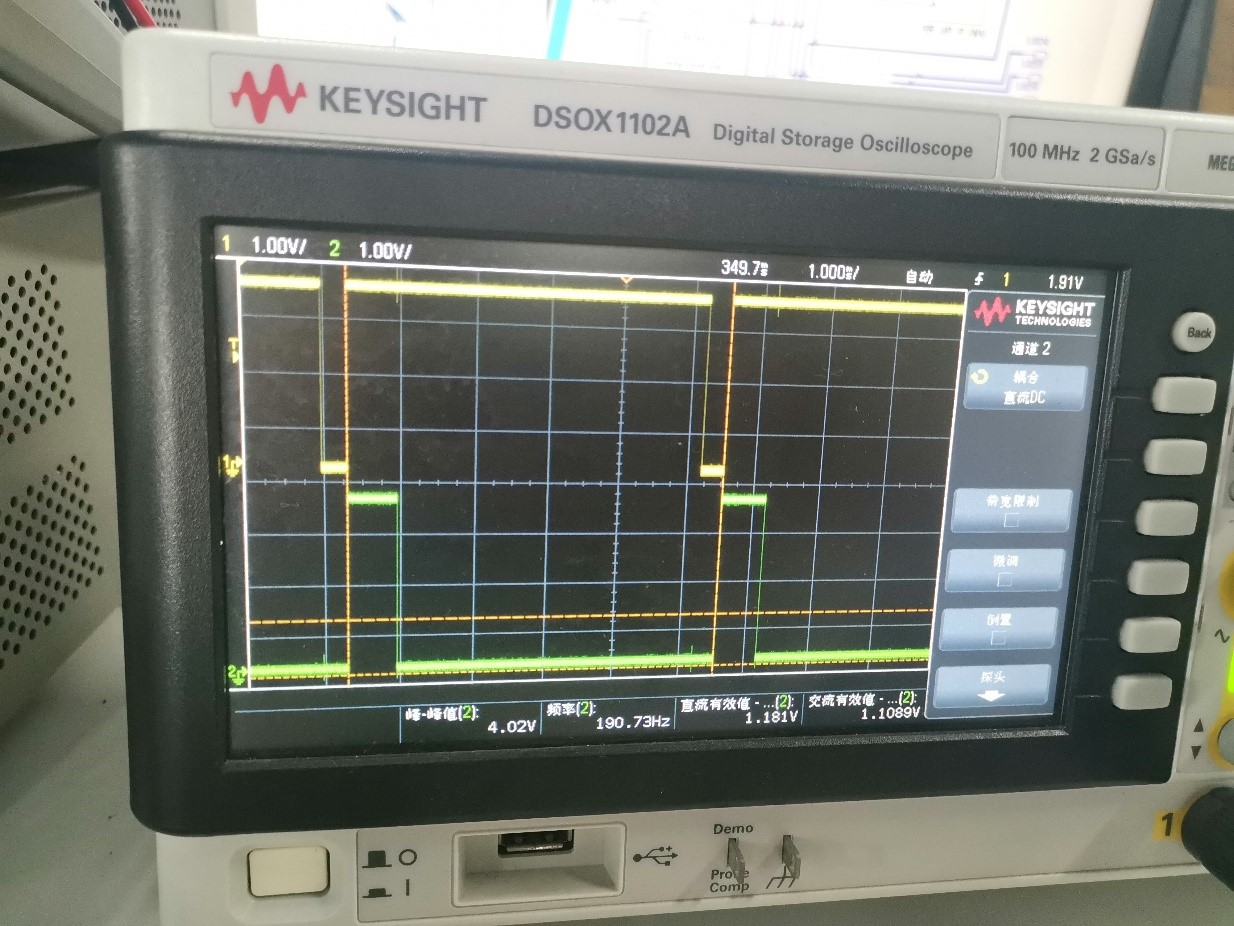
\includegraphics[width=0.45\textwidth]{pics/1S-V2/78.jpg}}
    \caption{移位寄存器单源周期触发测试-输出波形}
    \label{1S-V2 osci}
\end{figure}
可以看到在图(a)~(d)中,随着开关位置的变化,移位寄存器最高位的输出波形(通道2,绿色)随之相较移位寄存器置数信号位置依次向后移动,反映了移位寄存器数据移位的功能特点。在多输入时,可以看到移位寄存器将并行输入转换成为了串行输出。图(g)中的输入数据为我的学号。




\section{实验总结}
\begin{enumerate}
    \item 了解了计数器的基本工作原理与输出波形
    \item 掌握了利用已有计数器模块实现不同数值计数器的方法
    \item 利用计数器设计实现了秒表
\end{enumerate}

\section*{原始数据}



\end{document}